\chapter{The Kingdom, the Power, and the Glory}
\vspace{0.6cm}
\begin{center}
\nopagebreak
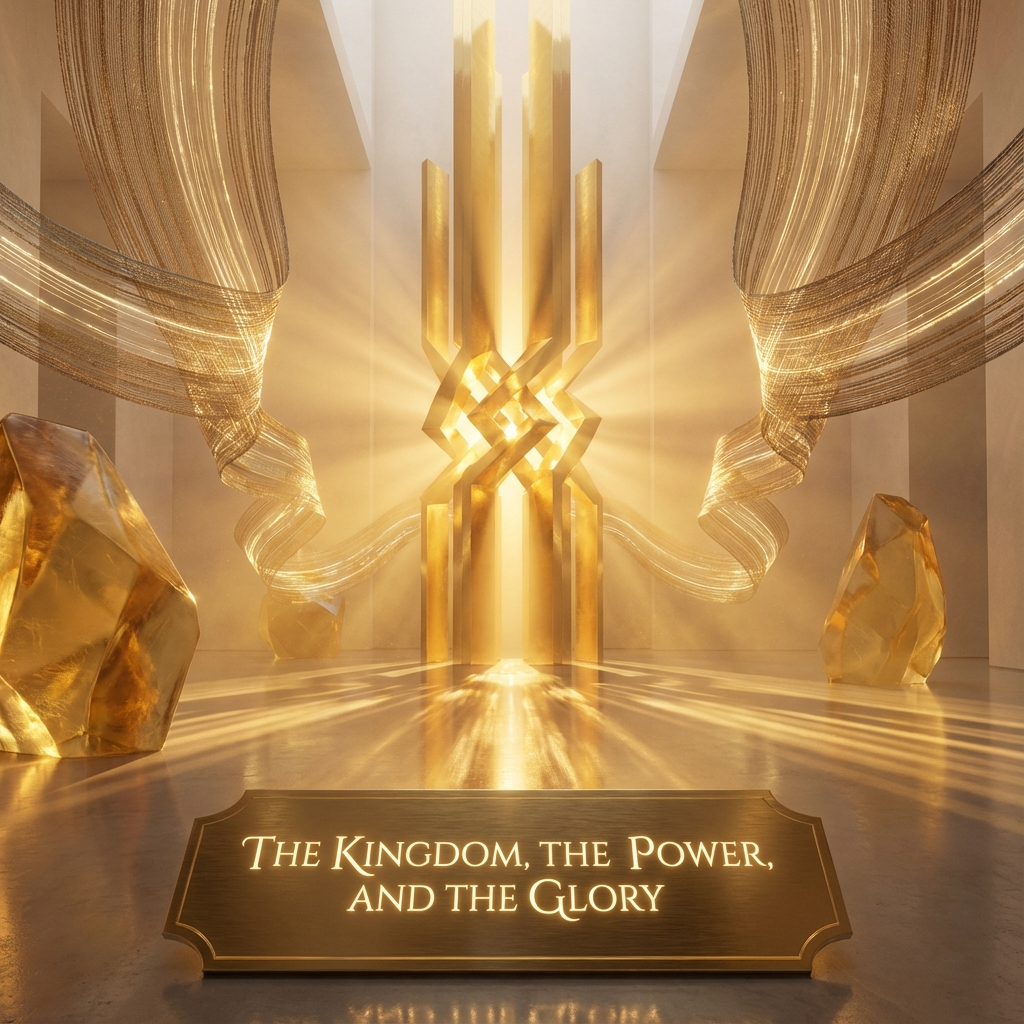
\includegraphics[width=0.75\textwidth,cfbox=gray!60 0.6pt 4pt]{kingdom_power.png}\\
\vspace{4pt}
{\small\itshape The Kingdom, Power, and Glory: eternal resonance.}
\end{center}

\vspace{0.6cm}
The journey was coming to an end. We were sitting on a bench in Plaza de Oriente, in front of the Royal Palace.
—Yours is the Kingdom, the Power, and the Glory —Jesus said, looking at the imposing building—. But not that kingdom of stones and guards.


—Which one then?


—The Kingdom is your inner peace. The Power is your ability to choose your vibration in every moment, whatever happens outside. And the Glory... the Glory is the joy of being who you are. Of being a child of the Universe.


He got up and stretched out his arms, as if embracing the world.
—Do not look for power outside. Do not look for people to applaud you. True power is silent. It is the certainty that you are never alone, that Life sustains you. When you understand that, when you feel it in your cells, you are already in the Kingdom. Here and now. Between Madrid, Las Rozas and Colmenarejo. The Kingdom is where you are, if you are awake.


He looked at me with an intensity that pierced my soul.
—Do not forget this, Francisco. You have the power. Use it to vibrate high. Use it to illuminate your corner of the world. That is your only task.